% latex
% bibtex journal
% bibtex conf
% bibtex techreport
% bibtex submitpaper
% latex
% # embedd the fonts
% dvips -j0 -Ppdf -Pdownload35 -G0 kbunte_thesis.dvi
% ps2pdf14 -dPDFSETTINGS=/prepress -dEmbedAllFonts=true kbunte_thesis.ps
% pdffonts
%%% For a B5 format, use the following option  
\documentclass[10pt,fleqn]{phdthesis}%,makeidx
\makeatletter
\renewenvironment{thebibliography}[1]
     {\@mkboth{\MakeUppercase\bibname}{\MakeUppercase\bibname}%
      \list{\@biblabel{\@arabic\c@enumiv}}%
           {\settowidth\labelwidth{\@biblabel{#1}}%
            \leftmargin\labelwidth
            \advance\leftmargin\labelsep
            \@openbib@code
            \usecounter{enumiv}%
            \let\p@enumiv\@empty
            \renewcommand\theenumiv{\@arabic\c@enumiv}}%
      \sloppy
      \clubpenalty4000
      \@clubpenalty \clubpenalty
      \widowpenalty4000%
      \sfcode`\.\@m}
     {\def\@noitemerr
       {\@latex@warning{Empty `thebibliography' environment}}%
      \endlist}
\makeatother
%%% For an A4 format, use there options instead
%\documentclass[12pt,makeidx]{phdthesis}
%\usepackage{a4wide}

%%% Fonts, uncomment only one option %%%
%\usepackage{utopia}
%\usepackage{charter}
\usepackage{palatino}
%\usepackage{newcent}
%\usepackage{avant}
%\usepackage{pifont}
%\usepackage{mathpple}
%\usepackage{mathptmx}

%%% If you want to use MakeIndex to create automatically
% an index, uncomment these lines
\usepackage{makeidx}     % only with Latex2e
\makeindex

% Other packages
%\usepackage{fancyheadings}
\usepackage{fancyhdr}
\usepackage{amsmath,dsfont}
\usepackage{amssymb,mathabx}
\usepackage{epsfig}
\usepackage[figbotcap]{subfigure}
% \usepackage{subfig}
\usepackage{graphics}
\usepackage{float}
\usepackage{here}
\usepackage[abbr]{harvard}
\usepackage{rotating}
\usepackage{multirow}
\usepackage{comment}
\usepackage{captionhack}
\usepackage{epigraph}
\usepackage{array,multirow,nicefrac}
\usepackage{appendix}
\usepackage{acronym}
\usepackage[chapter]{algorithm}
\usepackage{algorithmic}

% \usepackage{showframe}

\usepackage{lscape}
\usepackage[table]{xcolor}
\usepackage{tabularx,booktabs}
\usepackage{wrapfig}

\usepackage{pstricks,pst-node}
% \usepackage{pstricks-add}%pst-char,,pst-text,ae,pst-grad,pst-slpe
\usepackage{fancybox}
% \usepackage[dvips,margin=1cm]{geometry}
% \usepackage{lmodern,pst-node}
\usepackage{psfrag}

% \renewcommand{\thesubfigure}{} 

\usepackage{float,afterpage,dblfloatfix}%stfloats
% dblfloatfix fixes two floatpages after each other
    % Alter some LaTeX defaults for better treatment of figures:
    % See p.105 of "TeX Unbound" for suggested values.
    % See pp. 199-200 of Lamport's "LaTeX" book for details.
    %   General parameters, for ALL pages:
    \renewcommand{\topfraction}{0.9}	% max fraction of floats at top
    \renewcommand{\bottomfraction}{0.8}	% max fraction of floats at bottom
    %   Parameters for TEXT pages (not float pages):
    \setcounter{topnumber}{2}
    \setcounter{bottomnumber}{2}
    \setcounter{totalnumber}{4}     % 2 may work better
    \setcounter{dbltopnumber}{2}    % for 2-column pages
    \renewcommand{\dbltopfraction}{0.9}	% fit big float above 2-col. text
    \renewcommand{\textfraction}{0.07}	% allow minimal text w. figs
%   Parameters for FLOAT pages (not text pages):
    \renewcommand{\floatpagefraction}{0.7}	% require fuller float pages
	% N.B.: floatpagefraction MUST be less than topfraction !!
    \renewcommand{\dblfloatpagefraction}{0.7}	% require fuller float pages

\makeatletter
\def\zaptype#1{%
\listsubcaptions % Finish the last set of sub-floats before
\def\@captype{#1}}% switching to another float type.
\makeatother

%%% Path to the directorz containing the graphics and figures 
\graphicspath{{./pics/},{./pics/chapter_2/},{./pics/chapter_3/},{./pics/chapter_4/},{./pics/chapter_5/},{./pics/chapter_6/}
,{./pics/chapter_7/},{./pics/chapter_8/},{./pics/chapter_9/}}
\usepackage{ifpdf}
\ifpdf
\graphicspath{{./png/}}
\DeclareGraphicsExtensions{.png}
\else
  \DeclareGraphicsExtensions{{.eps},{.epsi}}%,{.ps}
\fi
%%% General page formatting
\renewcommand{\textfraction}{0.01}
\renewcommand{\topfraction}{0.99}
\renewcommand{\floatpagefraction}{0.99}
\renewcommand{\bottomfraction}{0.99}

\newenvironment{Abstract}
{\begin{center}\textbf{Abstract}%
 \end{center} \small \it \begin{quote}}
{\end{quote}}

% Macro for 'List of Symbols', 'List of Notations' etc...
\def\listofsymbols{%%%%%%%%%%%%%%%%%%%%%%%
%Sample List of Symbols
%%%%%%%%%%%%%%%%%%%%%%%
% \vfill
\begin{tabbing}
% YOU NEED TO ADD THE FIRST ONE MANUALLY TO ADJUST THE TABBING AND SPACES
% $n$~~~~~\=\parbox{4.8in}{Vector size\dotfill \pageref{symbol:nml}}\\
$\C{X}$~~~~~~~~~\=\parbox{4.6in}{input space\dotfill \pageref{symbol:X}}\\
%ADD THE REST OF SYMBOLS WITH THE HELP OF MACRO
\addsymbol n: {number of input vectors}{symbol:n}
\addsymbol \v{x}^i: {$i$-th example}{symbol:x^i}
\addsymbol y^i: {$i$-th label}{symbol:y^i}
\addsymbol N: {dimensionality of the data}{symbol:N}
\addsymbol C: {number of classes}{symbol:C}
\addsymbol \v{w}^j: {$j$-th prototype}{symbol:w^j}
\addsymbol c(\v{w}^j): {class of $j$-th prototype}{symbol:c(w^j)}
\addsymbol n_{\v{w}}: {number of prototypes}{symbol:n_w}
\addsymbol d: {dissimilarity measure}{symbol:d}
\addsymbol R^i: {receptive field of prototype $\v{w}^i$}{symbol:R^i}
% \addsymbol E: {cost function}{symbol:E}
% \addsymbol \Phi: {scaling function}{symbol:Phi}
% \addsymbol \mu: {relative difference distance}{symbol:mu}
% \addsymbol \v{\lambda}: {relevance vector}{symbol:lambda}
% \addsymbol \v{\lambda}^j: {local relevance vector}{symbol:lambda^j}
% \addsymbol \Lambda: {relevance matrix (GMLVQ)}{symbol:Lambda}
% \addsymbol \Omega: {self-affine transformation (GMLVQ)}{symbol:Omega}
% \addsymbol \Lambda^j: {local relevance matrix (LGMLVQ)}{symbol:Lambda_j}
% \addsymbol \Omega^j: {local transformation (LGMLVQ)}{symbol:Omega_j}
% \addsymbol \kappa: {number of target neighbors (LMNN)}{symbol:kappa}
% \addsymbol Y: {matrix indicating same class memberships (LMNN)}{symbol:Y}
% \addsymbol X: {matrix containing the perimeter of invasion (LMNN)}{symbol:XLMNN}
% \addsymbol \Gamma: {relevance matrix (LMNN)}{symbol:Gamma}
% \addsymbol \Upsilon : {transformation matrix (LMNN)}{symbol:Upsilon}
\addsymbol M: {target dimension of dimension reduction}{symbol:M}
% ALWAYS KEEP THE FOLLOWING LINE
\end{tabbing} \clearpage}
\def\addsymbol #1: #2#3{$#1$ \> \parbox{4.6in}{#2 \dotfill \pageref{#3}}\\}
\def\newnot#1{\label{#1}} 


\pdfcompresslevel=3

\typeout{Dissertation}

\usepackage{hyperref}
\usepackage[resetlabels]{multibib}%[resetlabels]
% \def\@mb@citenamelist{cite,citep,citet,citealp,citealt,footcite,nocite}

% Initialize each paper type for which you need a bibliography.
% Just a dummy parameter is necessary.
% \newcites{p}{Publications}
\newcites{journal,conf,techreport,submitpaper}{Journal Papers,Conference Papers,Technical Reports, Submitted Papers}%Journal Papers

%%% To compile only one or some chapters, use the following
%   command 
%\includeonly{z_example_chapter1}
%\includeonly{thesis_acknowledgements,chapter2,chapter3}
% \includeonly{chapter6}

% Morerow Comments
% \newcommand{\comment}[1]{{}} 

%% special characters
% \def\bbbr{{\rm I\!R}} %reelle Zahlen
\newcommand{\R}{{\rm I\!R}}
\renewcommand{\v}[1]{\vec{#1}}
\newcommand{\C}[1]{\mathcal{#1}}
\renewcommand{\vec}[1]{\boldsymbol{#1}}
\newcommand{\m}[1]{\mathbf{#1}}
\newcommand{\Comp}{\mathds{C}}
\newcommand{\convolve}{\convolution}
\newcommand{\vs}{\varsigma}
\newcommand{\s}{\sigma}
\newcommand{\D}{\mathrm{D}}
\renewcommand{\t}[1]{\tilde{#1}}

% correct bad hyphenation here
% TODO hyphenation
\usepackage{hyphenat}
\hyphenation{qua-dra-tic SRBCT pre-ser-va-tion Min-kow-ski a-dapt-ive de-ri-va-tive pat-ches pre-serv-ing re-sul-ting Em-bedd-ing 
where-by uni-form de-ri-va-ti-ves con-ti-nu-ous-ly wille-keurige voor-ge-steld}
% solve hyphenation that contain a dash like electromagnetic-endioscopy: electromagnetic\hyp{}endioscopy
% high\hyp{}dimensional

% \usepackage{scrwfile}
% \usepackage{xy}%etex
% \xyoption{all} 

%%% Begining of the document 
\begin{document}
% TODO 
% acronyms
\acrodef{LVQ}{Learning Vector Quantization}
\acrodef{OLVQ1}{optimized learning-rate LVQ}
\acrodef{RLVQ}{Relevance LVQ}
\acrodef{GLVQ}{Generalized LVQ}
\acrodef{GRLVQ}{Generalized Relevance LVQ}
\acrodef{LGRLVQ}{Localized GRLVQ}
\acrodef{GMLVQ}{Generalized Matrix LVQ}
\acrodef{LGMLVQ}{Localized GMLVQ}
\acrodef{LiRaM LVQ}{Limited Rank Matrix LVQ}
\acrodef{LLiRaM LVQ}{Localized LiRaM LVQ}
\acrodef{CIA LVQ}{Color Image Analysis LVQ}

\acrodef{STD}{standard deviation}
\acrodef{MVN}{Multivariate Normal density}
\acrodef{1-NN}{Nearest Neighbor}
\acrodef{$k$-NN}{$k$-Nearest Neighbor}
\acrodef{LMNN}{Large Margin Nearest Neighbor}
\acrodef{SDP}{semidefinite program}
\acrodef{MLE}{Maximum Likelihood Estimation}

\acrodef{SOM}{Self-organizing Map}
\acrodef{GSOM}{Growing Self-Organized Map}
\acrodef{NG}{Neural Gas}
\acrodef{ANN}{Artificial Neural Network}
\acrodef{SVM}{Support Vector Machine}
\acrodef{CBIR}{Content Based Image Retrieval}
\acrodef{XOM}{Exploration Observation Machine}
\acrodef{SONE}{Self Organized Neighbor Embedding}
\acrodef{t-SONE}{t-distributed SONE}

\acrodef{PCA}{Principal Component Analysis}
\acrodef{NCA}{Neighborhood Component Analysis}
\acrodef{LDA}{Linear Discriminant Analysis}
\acrodef{FDA}{Fisher Discriminant Analysis}
\acrodef{LFDA}{local Fisher discriminant analysis}
\acrodef{PLS}{partial Least Squares regression}
\acrodef{MDS}{Multidimensional Scaling}
\acrodef{SNE}{Stochastic Neighbor Embedding}
\acrodef{t-SNE}{t-distributed SNE}
\acrodef{LPP}{Locality\hyp{}Preserving Projection}
\acrodef{TPP}{Targeted Projection Pursuit}
\acrodef{LLE}{Locally Linear Embedding}
\acrodef{MVU}{Maximum Variance Unfolding}
\acrodef{LLC}{Locally Linear Coordination}
\acrodef{NeRV}{Neighborhood Retrieval Visualizer}
\acrodef{t-NeRV}{t-distributed NeRV}
\acrodef{LTSA}{Local Tangent Space Alignment}

\acrodef{sNeRV}{supervised NeRV}
\acrodef{MRE}{Multiple Relational Embedding}
\acrodef{cMVU}{Colored MVU}
\acrodef{MUHSIC}{maximum unfolding via Hilbert-Schmidt independence criterion}
\acrodef{S-Isomap}{supervised Isomap}
\acrodef{PE}{Parametric Embedding}

\acrodef{KL}{Kullback-Leibler}
\acrodef{GKL}{generalized Kullback-Leibler}
\acrodef{IS}{Itakura-Saito}

\pagestyle{fancyplain}
\pagenumbering{roman}

%%%  \include the `front matter'
%\thispagestyle{empty}

\begin{center}

\vspace*{1cm}

{\LARGE \textbf{Adaptive Dissimilarity Measures,\\[.5cm]Dimension Reduction and Visualization}}


\vspace*{13cm}

{\large Kerstin Bunte}
\end{center}

\clearpage

\thispagestyle{empty}
\noindent {\bf Book cover:} Isosurfaces of different dissimilarity measures on a glass surface:\\
\begin{tabular*}{1\textwidth}{@{\extracolsep{\fill}} @{}r p{0.73\textwidth}}
% \begin{tabular}{@{}rl}
Front (right to left): & Minkowski metric with $p=1$ and isolevel 0.3 and Itakura-Saito divergence with
isolevel 0.2.\\
Back (right to left): & Gamma-divergence with $\gamma=1.5$ and isolevel 0.02 and Minkowski metric with $p=3$ and isolevel
0.3.
% \end{tabular}
\end{tabular*}
Alternative and adaptive similarity measures are discussed in this thesis.

\vfill

\noindent 
% ISBN: 978-90-367-5186-5
\\
\\
Published by \emph{Atto Producties Europe} - www.attoproducties.nl - {\small Groningen}
% \\ \\
% www.attoproducties.nl
\\\\%[0.5cm]
supported by the Netherlands Organisation for Scientific Research (NWO)\\
under project number 612.066.620\\
% \begin{wrapfigure}{r}{0.5\textwidth}
\parbox{0.35\textwidth}{\hfill}
\parbox[r]{0.65\textwidth}{%\frame{
% \includegraphics{2d_NWO_LogoBasis_Zw}

\includegraphics{pics/2b_NWO_LogoBasis_CMYK.eps}%}
}
% \end{wrapfigure}

\cleardoublepage

\thispagestyle{empty}

\parbox[t][0.99\textheight][s]{1\textwidth}{
\centering

\large

{\bf RIJKSUNIVERSITEIT GRONINGEN}

\vspace*{1cm}

\textbf{Adaptive Dissimilarity Measures,\\[.05cm]
Dimension Reduction and Visualization}

\vfill

{\bf Proefschrift}

\bigskip
ter verkrijging van het doctoraat in de\\
Wiskunde en Natuurwetenschappen\\
aan de Rijksuniversiteit Groningen\\
op gezag van de\\
Rector Magnificus, dr.\ E.~Sterken,\\
in het openbaar te verdedigen op\\
vrijdag 16 december 2011\\% maandag 14 juni
om 12.45 uur%14.45 uur
\\
\vfill
door
\vfill
\textbf{Kerstin Bunte}\\
\vfill
\vspace*{-0.1cm}geboren op 6 september 1981\\
te Bielefeld, Duitsland
}

\newpage

\thispagestyle{empty}

%\begin{flushleft}

\noindent
\begin{tabular}{@{}ll}
% \!\!\!
Promotores:             	& Prof.\ dr.\ M. Biehl\\
             			& Prof.\ dr.\ N. Petkov
\\
\\
% \!\!\!
Beoordelingscommissie:  	& Prof.\ dr.\ E. Mer\'{e}nyi\\ 
                        	& Prof.\ dr.\ M. Opper\\ 
                        	& Prof.\ dr.\ M. Verleysen\\ 
\end{tabular}


\vfill

\noindent
ISBN: 978-90-367-5186-5
\\

%\end{flushleft}

%\include{thesis_dedication}

%% create the table of contents
\cleardoublepage
%\clearpage
\lhead[]{\fancyplain{}{\rightmark}}
\chead[\fancyplain{}{}]{\fancyplain{}{}}
\rhead[\fancyplain{}{\leftmark}]{\fancyplain{}{}}
%\rhead[\fancyplain{}{}]{\fancyplain{}{}}
%\lhead[\fancyplain{}{}]{\fancyplain{}{}}
\tableofcontents

%%  add the acknowledgements to the table of contents
\cleardoublepage
\addcontentsline{toc}{chapter}{Acknowledgements}
\chapter*{Acknowledgments}
\pagestyle{empty}

\vspace{-1cm} 


{\flushright Kerstin Bunte\\ Groningen\\ \today\\ }


\begin{thesymbols}
\listofsymbols
\end{thesymbols}

\addcontentsline{toc}{chapter}{List of figures}
\listoffigures
% \addcontentsline{toc}{chapter}{List of tables}
% \listoftables
\addcontentsline{toc}{chapter}{List of algorithms}
\listofalgorithms

%\clearpage
\cleardoublepage

%%% Customisation of the header and footer for the chapters
\pagestyle{headings}
%------------------------------
\newcommand{\publ}{}

\pagestyle{fancyplain}
%\setlength{\headrulewidth}{0.3pt}
%\setlength{\footrulewidth}{0.0pt}
%\setlength{\plainfootrulewidth}{0.0pt}
%\setlength{\plainheadrulewidth}{0pt}
\renewcommand{\sectionmark}[1]{\markright{\it \thesection.\ #1}}
\renewcommand{\chaptermark}[1]{\markboth{
       \it \thechapter.\ #1}{}}
\lhead[\thepage]{\fancyplain{}{\rightmark}}%\publ
\chead[\fancyplain{}{}]{\fancyplain{}{}}
\rhead[\fancyplain{}{\leftmark}]{\fancyplain{}{\thepage}}
\lfoot[]{}
\cfoot[]{}
\rfoot[]{}
%------------------------------


%%  include the LaTeX files containing the text for each chapters 
%   create the appendix and include it 
\pagenumbering{arabic}

% \noappendicestocpagenum
% \addappheadtotoc
\renewcommand{\publ}{}

% \index{Classification!LVQ}

\chapter{Introduction}

\PARstart{D}ue to advanced sensor technology, rapidly increasing digitalization capabilities and the availability of less and 
less expensive storage volume the amount of data has grown tremendously in the last decades. 
In the years between 1999 and 2002 an increase of stored information about 30\% each year was estimated \cite{Lyman2003}. 
Usually this data consists of a variety of measured features leading to also very high dimensional data sets. 
Manually inspection of the data becomes more costly and automatic methods to help humans to quickly scan through 
massive data amounts are desirable. 
This gave rise to many applications in computer science to process the available data: 
advanced techniques including data mining \cite{Han2005}, pattern recognition \cite{Duda2000} and machine learning 
\cite{Mitchell1997,Ripley1996,Bishop2007}, among others. 
Even with great progress in those fields the optimization of existing methods and development of novel schemes is highly 
desirable to perform faster and more efficient data analysis. 

The field of machine learning concerns the design of algorithms, 
which aim at the optimization of adaptive systems on the basis of example data. 
A model is adapted to learn complex patterns and process new data coming from the same domain better regarding the specified objective. 
The analysis of patterns involves a number of tasks including data representation, classification, clustering, density estimation, 
regression, feature extraction and dimension reduction, just to name a few. 
A lot of data visualization tools have been developed to use cognitive capabilities of humans for structure 
detection in visual images. 
Structural characteristics of the data can be captured almost instantly by humans despite the amount of data points which 
are represented in the visualization. 
Hence, dimension reduction and visualization are commonly used modern data mining techniques \cite{Lee2007}. 
Machine learning is broadly categorized into reinforcement, supervised and unsupervised learning. 
Reinforcement learning is inspired by behaviorist psychology and concerns the finding of suitable actions to maximize some notion 
of reward \cite{Sutton1998}. 
Supervised techniques involve external supervision, which provides correct responses to the given inputs. 
The aim is usually the discrimination of the categories and to maximize the generalization for novel data. 
Unsupervised methods, on the other hand, do not need supervision and their goal is the discovery of underlying structures 
and regularities based on the definition of some basic properties of the data.
An elaborate description concerning the history of machine learning can be found in, e.\ g. 
\cite{Bishop1995,Ripley1996,Mitchell1997,Duda2000,Bishop2007}. 

A very intuitive supervised technique called \ac{$k$-NN} classifier compares the unknown data to all known examples with 
respect to some dissimilarity measure \cite{Duda2000}. 
Obviously the computational effort and memory usage scales with the number of known samples. 
Therefore prototype-based techniques were developed, which employ representations of data subsets. 
The prototypes are vector locations in the feature space. 
They usually serve as typical representatives and reflect the characteristics of the data in their direct neighborhood. 
% Supervised and unsupervised methods can be used to represent the data by means of prototypes. 
Some prominent unsupervised examples are the \ac{SOM} \cite{Kohonen2001} and \ac{NG} \cite{Martinetz1991}. 
And a popular supervised family of such prototype-based classification methods is \ac{LVQ} \cite{Kohonen2001}. 
% The set of prototypes and the dissimilarity measure parameterize the model. 
All these methods crucially depend on the distance measure, which is used to adapt the prototype positions and 
performs the nearest prototype classification. 
Therefore the learning of adaptive metrics with respect to the given problem at hand was investigated \cite{Xing2002,Chopra2005,Frome2007,Schneider2009a,Schneider2009b}. 

This thesis investigates adaptive dissimilarities and applications varying from classification up to supervised and unsupervised 
dimension reduction. 

\section{Scope of this thesis}

The objective of this thesis is manifold, it contains:
\begin{itemize}
\item the introduction of prototype-based adaptive dissimilarity learning with limited rank matrices, 
\item a new method based on that principle for learning in complex valued data domains and 
\item a general view and new algorithms for unsupervised as well as supervised dimension reduction and visualization. 
\end{itemize}
%for prototype-based adaptive dissimilarity learning
Adaptive dissimilarities are a powerful tool, which are shown to improve the performance of supervised methods, such as 
for example \ac{LVQ} and the \ac{$k$-NN} classifiers. 
These classification algorithms crucially depend on the distance measure used. 
Metric adaptation techniques allow the learning of discriminative dissimilarity measures from a given set of representative example data. 
Restrictions in adaptive matrix learning, e.\ g. the limitation of the rank, enables  
the learning of discriminative global or local linear transformations. 
These transformations can then be used for supervised dimension reduction and visualization. 
It also reduces the number of the effective learning parameters, 
which might be interesting from the computational point of view. 

In the first part of this contribution previously proposed methods for metric learning in \ac{LVQ} are extended to limited rank matrices. 
Several practical applications are investigated including \ac{CBIR}, dimension reduction and visualization. 
Furthermore we provide an extension which can be used on complex valued data shown on an example for texture classification in images. 

The second part of this thesis focuses on dimension reduction and visualization. 
We provide a general view on existing dimension reduction methods, 
which originally provide just an implicit mapping of the given data points itself. 
Based on this general principle we extend these methods to learn the parameters of explicit mapping functions instead. 
This provides direct out-of-sample extensions, reduces computational effort by restricting the learning process just on a small 
subset of the possible large data set and enables the formal investigation of the generalization ability. 
Furthermore we provide an unsupervised dimension reduction method, which in contrast to other techniques exhibit 
a complexity which scales linear with the number of data points in every step. 
It aims in the combination of fast online learning with the high quality of direct divergence optimization, 
successfully used by state-of-the-art techniques.  

\section{Outline}

% This section briefly addresses the outline of the thesis and the topics of the chapters. 
% The thesis is divided into two parts.  
% Part \ref{part:1} spans from Chapters 2 to 4 and  discusses adaptive dissimilarity measures especially as extensions of \ac{LVQ}. 
% The metric learning defined in this work can be reformulated to learn global or local linear projections of 
% the data, which smoothly leads over to Part \ref{part:2} of the thesis dealing with dimension reduction. 
% 
% The chapters are organized as follows: 
% Chapter \ref{chapter:LVQ} provides a short introduction to prototype-based learning and adaptive dissimilarities. 
% Basic algorithms like \ac{GLVQ} and \ac{GMLVQ} are described in detail. 
% The metric adaptation scheme is then modified to use limited rank matrices, which reduce the number of parameters and 
% thus the computational effort and gives direct access to supervised dimension reduction. 
% The latter aspect is resumed and investigated in more detail in Chapter \ref{chapter:discriminative_DR} 
% in the second part of this thesis. 
% 
% In Chapter \ref{chapter:CBIR} adaptive dissimilarity learning is used in an application for \ac{CBIR} in Dermatology.  
% The aim is a computer aided diagnosis system which helps the user, e.\ g. medical doctors, with targeted searches in image data bases. 
% A learned discriminative distance measure is used to retrieve an arbitrary number of most similar pictures from a data base of images 
% of skin lesions. 
% Two methods for metric learning are used and compared: \ac{LMNN}, which bases on the \ac{$k$-NN} algorithm, and the \ac{LVQ} based
% approach. 
% It is shown, that adaptive dissimilarities can be used to improve the performance of a \ac{CBIR} system. 
% 
% Chapter \ref{chapter:CIA_LVQ} introduces a variant of \ac{LVQ} defined on complex valued data. 
% The modification is shown on one example application for texture classification in color images. 
% These variant called \ac{CIA LVQ} combines well known image analysis filter techniques with prototype-based transformation learning 
% defined in the Fourier domain. 
% 
% % The introduction to the second part of the thesis concerning 
% Chapter \ref{chapter:DiReduct} provides an introduction to the second part of the thesis: dimension reduction and visualization. 
% An overview over existing techniques is given and a general principle is formulated. 
% Based on that principle a general framework is proposed which extends given dimension reduction techniques to learn an 
% explicit mapping function. 
% This way those methods, which are originally introduced to provide implicit point-to-point embeddings can 
% be extended to learn mapping functions instead. 
% Out-of-Sample extensions become immediate, the investigation of the generalization ability is possible and it can save computational 
% effort, because the mapping function can be learned on a representative small subset of the data. 
% 
% In Chapter \ref{chapter:discriminative_DR} the adaptive distances and discriminative transformations introduced in Chapter 
% \ref{chapter:LVQ} are used for supervised dimension reduction and visualization. 
% A variety of given unsupervised techniques are extended to use label information by plugging in the supervised learned 
% distance or the local linear transformations. 
% 
% Most dimension reduction techniques preserve properties extracted from local neighborhoods. 
% This requires the computation of pairwise distances, so the computational effort squares with the number of points. 
% Chapter \ref{chapter:SONE} introduces a dimension reduction method which combines the high performance of 
% direct divergence optimization with fast online learning, leading to a complexity growing linear with the number of points. 
% There are numerous divergences offering different properties. Chapter \ref{chapter:divergences} gives an overview over the three
% divergence
% families and examples thereof. Using the concept of Fr\'{e}chet derivatives three algorithms are expanded to the use of arbitrary
% divergences. 
% 
% Finally, Chapter \ref{chapter:conclusion} presents a brief summary of the research and a collection of ideas for future work and 
% investigation. 

% \begin{subappendices}
%  \include{appendix1}
% \end{subappendices} 

\part{Adaptive Dissimilarity Measures}%Metrics in Prototype Based Learning
\label{part:1}

\noappendicestocpagenum
% \addappheadtotoc
%%% Chapter heading commands %%%

%\setlength{\headheight}{1.2cm}

% \renewcommand{\publ}{\flushleft\footnotesize{Published as:\\[0.1cm]
% % K. Bunte, P. Schneider, B. Hammer, F.-M. Schleif, T. Villmann and M. Biehl -- \textit{``Discriminative Visualization by Limited Rank Matrix Learning,''} Leipzig University, Machine Learning Reports, no. 3, vol. 2, pp. 37--51, 2008.\\[0.1cm]
% K. Bunte, P. Schneider, B. Hammer, F.-M. Schleif, T. Villmann and M. Biehl -- \textit{``Limited Rank Matrix Learning Discriminative Dimension Reduction and Visualization,''} submitted to Neural Networks 2010.\\}}

\chapter{Distance Based Classification}%Learning Vector Quantization and Metric Adaptation
\label{chapter:LVQ}


\epigraph{Everything has its beauty but not everyone sees it.}{Confucius}

%%% Abstract %%%

\begin{Abstract}
This chapter introduces %the background in prototype based classification schemes
the basic \acf{LVQ} algorithms and notations used throughout the thesis. 
We discuss nearest prototype classification and a set of \ac{LVQ} learning schemes, 
which are relevant in the context of this work. 
Furthermore we explain the concept of parameterized dissimilarity and metric adaptation proposed in the literature.
\end{Abstract}

%%% reset acronyms %%%
\acresetall 

\section{Introduction}
\label{sec:biological_aspects}

\PARstart{M}achine learning \cite{Mitchell1997,Bishop2007} constitutes a huge field in computer science 
expanding into broad distribution of both, application and theory. 
The term ``learning'' comprises the biological point of view by modeling the theory of psychologists of learning in animals and humans. 
And it also addresses the development of algorithms aiming at the adjustment to a given objective based on empirical data. 
Thus, from a given set of input/output pairs produced by an complicated unknown process a machine 
should be able to adjust its internal structure such that the correct output is reproduced for a large number of samples. 
This part of the thesis concentrates a subfield usually referred to as supervised learning: 
Samples are given for which the output is (sometimes only approximately) known. 
The aim is to find a hypothesis that closely agrees with these given data and generalizes well, 
i.e. produces the desired output also for new samples. 
% data mining aims in the finding of hidden relationships and correlations in big data sets. 

\ac{LVQ}\index{Classification!LVQ} and its variants constitute a popular family of supervised prototype-based classifiers. 
The basic algorithm introduced by \cite{Kohonen1986} is parameterized by a set of labeled prototypes 
representing the classes in the input space in combination with a dissimilarity measure. 
The classification takes places by a nearest prototype scheme, i.e. a new sample is assigned to the 
class represented by the closest prototype with respect to the given metric. 
These algorithms are naturally suitable for multi-class problems without changing the learning rules and the complexity is usually 
dependent on the number of prototypes and only indirect on the number of classes. 
This classification procedure is closely related to the popular \ac{$k$-NN} approach \cite{Cover1967}, 
which keeps the given labeled data set as a reference set and classifies every new data point to the class 
given by the majority among its $k$ nearest neighbors. 
Although the \ac{$k$-NN}\index{Classification!$k$-NN}
 approach is one of the most intuitive and simplest classification algorithms it shows often very good performance. 
Nevertheless, it might become very expensive in memory usage and computation for very large reference sets. 
Prototype methods overcome those problems by defining a clustering on the data. 
Another advantage of \ac{LVQ} is the interpretability of the resulting parameters: 
It does not suffer from a ``black box'' character like an \ac{ANN} or a \ac{SVM}. 
The prototypes reflect the characteristic class-specific attributes of the input samples. 
% This interpretability makes \ac{LVQ} especially attractive for complex real life applications, e.g. in bioinformatics, image analysis
% and in medical environments 

The basic heuristic algorithm, called LVQ1 \cite{Kohonen1986}, adapts a set of prototypes from labeled training 
data by implementing Hebbian learning steps. 
Additionally, Kohonen introduced two alternative learning schemes: \ac{OLVQ1} and LVQ2.1, aiming at faster convergence and better 
approximation of Bayesian decision boundaries, respectively. 
Furthermore, several \ac{LVQ} variants were proposed, which are derived from an explicit cost function
\cite{Sato1996,Seo2002,Seo2003}. 
Cost function based approaches are easily extended to a larger number of adaptive parameters. 
And methods of theoretical learning theory can be used to investigate risk bounds and convergence behavior. 
A mathematical analysis with respect to the cost function is performed in \cite{Sato1998} and the authors of \cite{Crammer2002} 
showed that \ac{LVQ} aims at margin optimization and therefore good generalization ability can be expected. 
Further theoretical analysis of different \ac{LVQ} variants and statistical physics investigations on simplified model situations 
can be found in \cite{Gosh2006,Biehl2007}.
Further extensions of the \ac{LVQ} classification scheme includes the combination with other prototype-based learning schemes. 
For example the comprehension of the neighborhood cooperation known from \ac{SOM} or \ac{NG} into the learning process 
\cite{Kohonen2002,Hammer2005}. 

% Euclidean distance popular choice ; Alternatives from information theory Mwebaze 2010 ; optimization of dissimilarity - metric learning ; 
% adaptive metrics
Particularly interesting for distance-based machine learning methods like mentioned before is the employed dissimilarity measure. 
A very common choice is the Euclidean distance, which is a special case of the Minkowski metric. 
Recently, also divergences known from information theory were used as dissimilarity measure in 
vector quantization schemes \cite{Mwebaze2011,Villmann2011}. 
In supervised settings where auxiliary information, such as labels, is available the adaptation of the distance 
by means of metric learning became popular. 
Some \ac{LVQ} variants have been proposed, which aim at the optimization of the distance measure for a specific application 
\cite{Bojer2001,Hammer2002,Schneider2009a,Schneider2009b}. 
Also methods which aim at the optimization of the \ac{$k$-NN} classification scheme have been developed using adaptive 
dissimilarities \cite{Goldberger2004,Weinberger2006}. 
Usually a big improvement of the classification performance can be observed when metric learning is incorporated in the algorithms. 
In the following section we will review some machine learning techniques used throughout the thesis, 
especially, existing metric adaptation schemes are presented. 

% \section{Algorithms}
\section{Nearest prototype classification}

We assume that the input data $\C{X}$\newnot{symbol:X} consists of $n$\newnot{symbol:n} examples 
$\{\v{x}^i\}_{i=1}^n\in\R^N$\newnot{symbol:x^i}\newnot{symbol:N} together with their corresponding labels 
$y^i\in\{1,\dots, C\}$\newnot{symbol:y^i}\newnot{symbol:C}, where $N$ denotes the dimension and $C$ the number of classes or categories. 
A nearest prototype classifier is parameterized by a set of labeled prototype vectors $\v{w}^j$, 
also called {\it codebook}, and a distance measure $d$\newnot{symbol:d}. 
The protoytpes $\v{w}^j$\newnot{symbol:w^j} are defined on the same feature space as the input data and they carry 
the label $c(\v{w}^j)$\newnot{symbol:c(w^j)} of the class they aim to represent. 
This implies the definition
\begin{equation}
\label{eq:W}
\mathbf{W} = \{ (\v{w}^j,c(\v{w}^j))\in \R^N \times\{1,\dots, C\}\}_{j=1}^{n_{\v{w}}}\enspace ,
\end{equation}
\newnot{symbol:n_w}where the number of prototypes $n_{\v{w}}\ge C$, which means that at least one prototype per class is needed. 
A popular distance measure is the Euclidean distance, which is a special case of the general Minkowski metric
\begin{figure}[tpb]
\centering
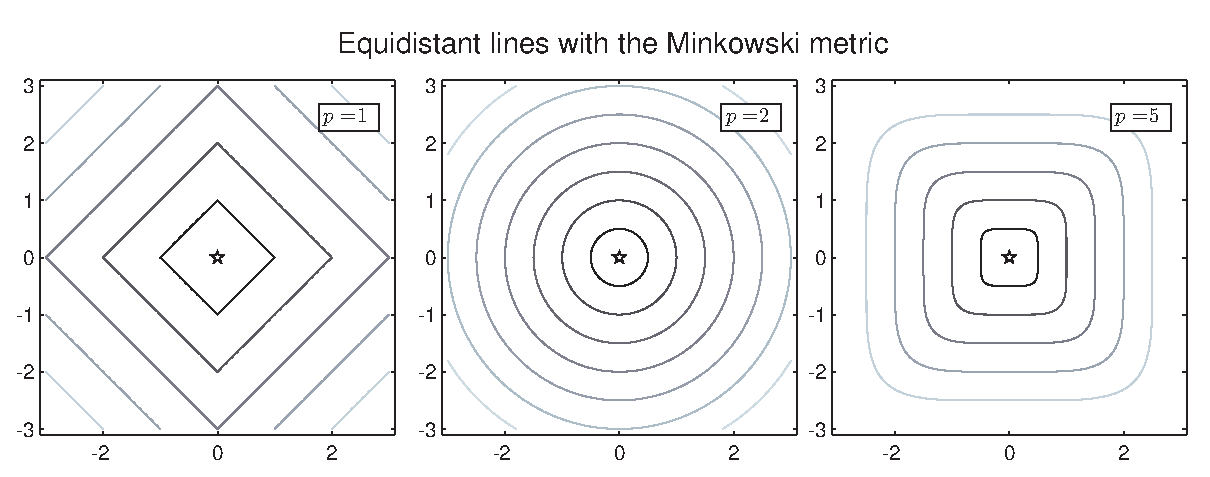
\includegraphics[width=\textwidth]{pics/minkowski_metrics.eps}%}
\caption[Equidistance lines using the Minkowski metric]{Visualization of the equidistance lines from the origin using the 
Minkowski metric with different values of $p$.}
\label{fig:Minkowski}
\end{figure}
\begin{equation}
\label{eq:minkowski}
 d^p(\v{x},\v{w}) = \left(\sum_{i=1}^N |x_i-w_i|^p\right)^\frac{1}{p}
\end{equation}
with $p=2$. 
Examples of the equidistance lines using the Minkowski metric and different values for $p$ are shown in Figure \ref{fig:Minkowski}. 
The classification takes places by a winner-takes-all scheme, i.e.\ a new data point $\v{x}$ is assigned to the class represented by 
the closest prototype:
\begin{equation}
\label{eq:nearest_prototype_classification}
 \v{x} \leftarrow c(\v{w}^i)\text{, with }\v{w}^i=\arg\underset{j}{\min}\ d(\v{x},\v{w}^j),
\end{equation}
braking ties arbitrary. The set of protoytpes and the metric is partitioning the input data space. 
Each prototype $\v{w}^i$ has a receptive field $R^i$\newnot{symbol:R^i}, which is a region in the feature space where $\v{w}^i$ 
is closer to the data than any other prototype:
\begin{equation}
\label{eq:Receptive_field_prototypes}
 R^i = \{ \v{x}\in \C{X}|\ d(\v{x},\v{w}^i)<d(\v{x},\v{w}^j), \forall i\neq j \} \enspace .
\end{equation}
Figure \ref{fig:NPC} shows two examples of nearest prototype classification on a three class problem using different distance measures. 
The Euclidean distance leads piecewise linear decision boundaries and receptive fields. 
For different values of $p$ in the Minkowski metric more general decision boundaries can be realized. 

The number of protoytpes is a hyper-parameter of the model and has to be optimized by means of a validation procedure.  
Too few prototypes may not represent the data structure sufficiently, which yields poor classification performance and 
too many prototypes may cause overfitting leading to poor generalization ability of the classifier. 
Many machine learning techniques have been proposed based on the nearest prototype classification scheme. 
Some of them used in the thesis will be addressed in the next sections. 

\begin{figure}[tpb]
\centering
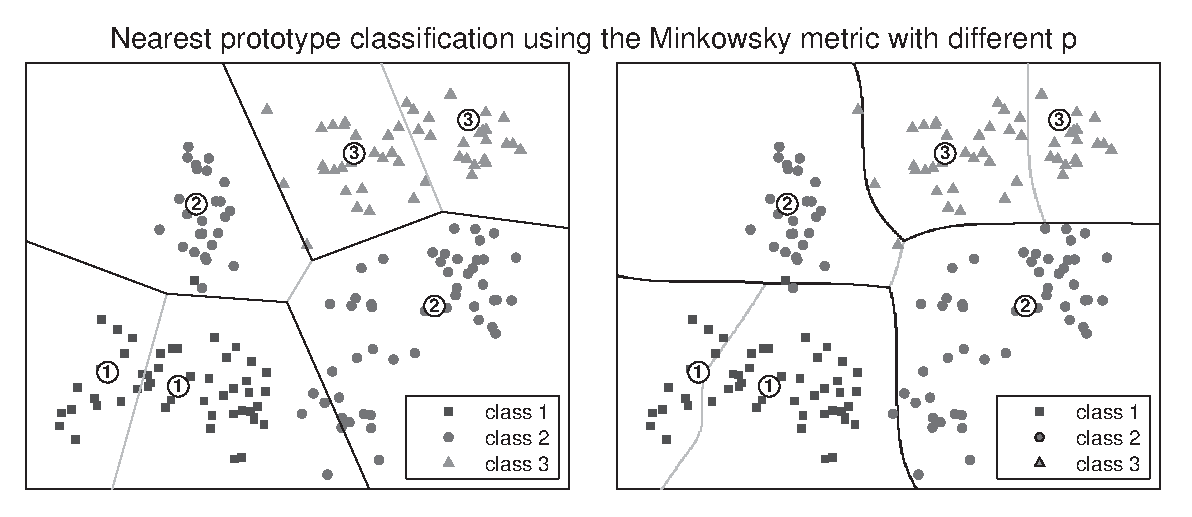
\includegraphics[width=\textwidth]{pics/NPC.eps}%}
\caption[Nearest prototype classification]{Visualization of the decision bounds of a nearest prototype classification scheme 
using different distances. The data is consisting of 3 classes and each class is represented by two prototypes. 
The Euclidean distance (left panel) shows piecewise linear boundaries where the gray lines denote the receptive fields of each prototype. 
In the right panel the Minkowski metric of order $p=5$ is used.% leading to nonlinear bounds.
}
\label{fig:NPC}
\end{figure}\index{Classification!Nearest prototype classification}
% \begin{subappendices}
%  \include{appendix2}
% \end{subappendices} 

\noappendicestocpagenum
\addappheadtotoc
%%% Chapter heading commands %%%

%\setlength{\headsep}{15pt}

\renewcommand{\publ}{\flushleft\footnotesize{Published as:\\[0.1cm]
K. Bunte, P. Schneider, B. Hammer, F.-M. Schleif, T. Villmann and M. Biehl -- \textit{``Discriminative Visualization by Limited Rank Matrix Learning,''} Leipzig University, Machine Learning Reports (2:3), %no.\ 3
% , vol. 2, 
pp. 37--51, 2008.\\[0.1cm]
K. Bunte, P. Schneider, B. Hammer, F.-M. Schleif, T. Villmann and M. Biehl -- \textit{``Limited Rank Matrix Learning Discriminative Dimension Reduction and Visualization,''} accepted for publication in Neural Networks 2011.\\}}

\chapter{Limited Rank Matrix LVQ}
\label{chapter:LiRaMLVQ}

\epigraph{Projection makes it possible.}{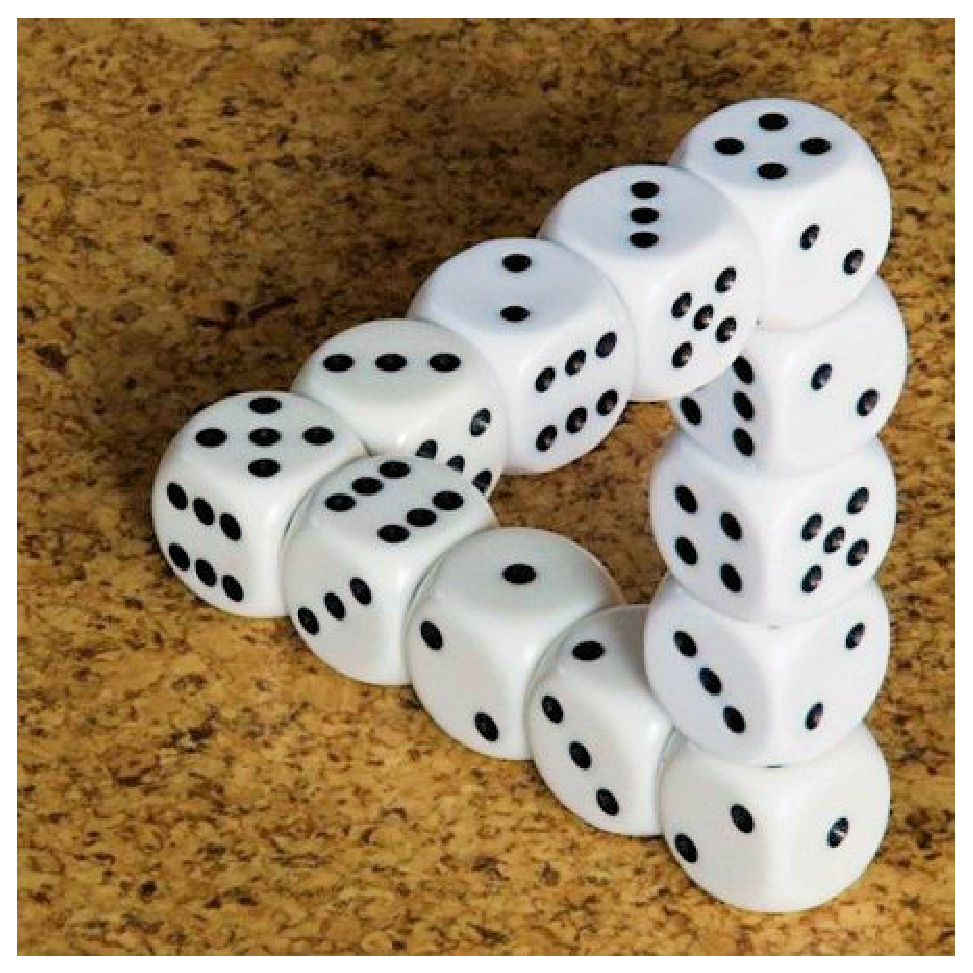
\includegraphics[width=2.5cm]{pics/dice_ShigeoFukuda.eps}\\The impossible triangle. Shigeo Fukuda}

\index{Adaptive Metrics}

%%% Abstract %%%

\begin{Abstract}
We present an extension of the %recently introduced 
Generalized Matrix Learning Vector Quantization algorithm. 
In the original scheme, adaptive square matrices of relevance factors parameterize a discriminative distance measure. 
We extend the scheme to matrices of limited rank corresponding to low-dimensional representations of the data. 
This allows to incorporate prior knowledge of the intrinsic dimension and to reduce the number of adaptive parameters efficiently. 
In particular, for very high dimensional data, the limitation of the rank can reduce computation time 
and memory requirements significantly. 
Furthermore, two- or three-dimensional representations constitute an efficient visualization method for labeled data sets. 
The identification of a suitable projection is not treated as a pre-processing step but as an integral part of the supervised training.  
Several real world data sets serve as illustration and demonstrate the usefulness of the suggested method.
\end{Abstract}

%%% Chapter sections %%%
% \index{Visual system}
% \iffalse
\section{Introduction}

\PARstart{I}n~\cite{Schneider2009a,Schneider2009b} the concept of \ac{GMLVQ} is introduced. 
% An important extension of this concept has been introduced in 
% in  the so-called Generalized Matrix LVQ (GMLVQ) a 
It uses the quadratic form Eq.\ (\ref{eq:d_Lambda}) as distance including a full matrix of relevances, 
which can account for correlations between different features. 
An adaptive self-affine transformation $\Omega$ (see Eq.\ (\ref{eq:Lambda})) of feature space identifies the coordinate 
system which is most suitable for the given classification task. 
The original formulation of \ac{GMLVQ} employs symmetric squared  matrices $\Omega\in\R^{N\times N}$ and 
is summarized in Algorithm \ref{alg:GMLVQ}. 
In the simplest case, one matrix is taken to define a global distance measure. 
Extensions to class-wise or local matrices, attached to individual prototypes Eq.\ (\ref{eq:d_Lambda_j}), 
are technically straightforward and allow for the parameterization of more complex decision boundaries. 

In this chapter we present and discuss an important modification: the use of rectangular transformation 
matrices $\Omega\in\R^{M\times N}$ with $M\le N$ \cite{MLR0308Bunte2008a,Bunte2011_LiRaMLVQ}%\cite{MLR0308Bunte2008a,Bunte_LiRaM_LVQ_2011}
.\newnot{symbol:M} 
The corresponding relevance matrices $\Lambda$ are of bounded rank $M$ or, in other words, distances are 
evaluated in a space with reduced dimension, see Eq.\ (\ref{eq:transformation}). 
The motivation for considering this variation of \ac{GMLVQ} is at least two-fold: 
% \begin{itemize}
% \item[(a)] 
(a) prior knowledge about the intrinsic dimension of the data can be incorporated efficiently and 
% \item[(b)] 
(b) the number of free parameters in the learning problem may be reduced significantly. 
% \end{itemize}

Although unrestricted \ac{GMLVQ} displays a tendency to reduce the rank of the relevance matrices in the training process, 
the advantages of restricting the rank explicitly are obvious. 
In particular for nominally very high-dimensional data, e.g.\ in image analysis or bioinformatics, 
unrestricted relevance matrices become intractable. 
In addition, optimization results can be poor when the search is performed in an unnecessarily large parameter space. 
Furthermore, the exact control of the rank allows for pre-defining the dimension of the intrinsic representation and 
is, for instance, suitable for the discriminative visualization of labeled data sets. 
In contrast with many other schemes that consider dimension reduction as a pre-processing step, our method
performs the training of prototypes and the identification of a suitable transformation simultaneously. 
Hence, both sub-tasks are guided by the ultimate goal of implementing the desired classification scheme.  

Appropriate projections into two- or three-dimensional spaces can furthermore be used for efficient visualization of labeled data. 
Visualization enables to use the astonishing cognitive capabilities of humans for visual perception when extracting 
information from large data volumes. 
Structural characteristics can be captured almost instantly by humans, independent of the number of displayed points. 
Classical unsupervised dimension reduction techniques represent data points contained in a
high dimensional data manifold by low dimensional counterparts in, for instance, two
or three dimensions, while preserving as much information as possible. 
Since it is not clear in advance which parts of the data are relevant to the user, this problem is inherently
ill-posed: depending on the specific data domain and the situation at hand, different aspects can be in the focus of attention. 
Prior knowledge, in form of label information, can be used to formulate a well-defined objective in terms of the 
classification performance. 

There exist a few classical dimensionality reduction tools which take class labels into account:
e.g.\ Classical Fisher \ac{LDA}, the recently introduced \ac{LFDA} \cite{Sugiyama2007}, 
\ac{NCA} \cite{Goldberger2004}, as well as \ac{PLS}. %offer supervised linear visualization techniques. 
\index{Dimension Reduction!Supervised methods!LDA}
\index{Dimension Reduction!Supervised methods!LFDA}
\index{Dimension Reduction!Supervised methods!PLS}
\index{Dimension Reduction!Supervised methods!NCA}
These methods can be extended to nonlinear projections by kernel methods \cite{Ma2007,Baudat2000}.  
% Kernel methods extend these settings to nonlinear projections \cite{Ma2007,Baudat2000}.
Adaptive dissimilarity measures which modify the metric %used for projection 
according to the given auxiliary information have been introduced e.g.\ in 
\cite{Kaski2001,Peltonen2004,Bunte_ESANN2009a,Bunte_CAIP2009_NLdimred,BunteESANNSI2009}.%,BunteESANNSI2009,
The resulting metric can be integrated into various techniques such as \ac{SOM}, \ac{MDS}, 
\index{Dimension Reduction!Unsupervised methods!SOM}
\index{Dimension Reduction!Unsupervised methods!MDS}or a recent information theoretic
model for data visualization \cite{Kaski2001,Peltonen2004,Venna2010}.
An ad hoc metric adaptation is used in \cite{Geng2005} to extend Isomap \cite{Tenenbaum2000} to class labels.
Alternative approaches change the cost function of dimensionality reduction, for instance 
by using conditional probabilities, class-wise similarity matrices 
or introducing a covariance-based coloring matrix for the side information as proposed in \cite{Iwata2007,Memisevic2005,Song2008}. 
The detailed explanation of the most important supervised and unsupervised dimension reduction techniques is 
given in Part \ref{part:2} %``Dimension Reduction and Visualization'' 
of this thesis. 

In the next section we describe the \ac{LiRaM LVQ} as extension of the original \ac{GMLVQ} formulation. 
%Sec.\ \ref{section:rectangular} we review GMLVQ in the following section.  
Afterwards we apply the novel approach to a benchmark problem and study the influence of the dimension 
reduction on the classification performance. 
We also compare the limited rank version to the naive approach of taking the first components of the full rank \ac{GMLVQ}. 
We show that reducing the rank after training not only requires more memory and CPU time, 
but also yields inferior classification performance compared to \ac{LiRaM LVQ}. 
In Sec.\ \ref{sec:LiRaM_LVQ_visualization} we present example applications of our algorithm in the visualization of labeled data. 
We also compare with visualizations obtained by \ac{LFDA} and \ac{NCA}. 
We conclude by summarizing our findings and providing an outlook on perspective investigations.
\begin{subappendices}
 % \begin{flushleft}
% {\bf\Large{{Appendices}}}
% \end{flushleft}
% \vspace{-.6cm}
% \section{Appendix: Derivatives}

\section{Derivatives of GMLVQ and LiRaM LVQ}\label{app:GMLVQ_derivatives}

Here we show the derivatives of the \ac{GMLVQ} costfunction $E_{\mathrm{GMLVQ}}$ for one presented training 
example $\v{x}^i$, see Eq.\ (\ref{eq:E_GMLVQ}), 
with respect to the prototypes $\v{w}^L$ with $L\in\{J,K\}$ and the transformation matrix $\Omega\in\R^{M\times N}$. 
The derivative with respect to the prototypes can be formulated like following:
\begin{align}
d^\Lambda_L &= \sum^N_r\sum^M_m\sum^N_n (x^i_r-w^L_r)\Omega_{mr}\Omega_{mn}(x^i_n-w^L_n) \\
% 
\frac{\partial E_{\mathrm{GMLVQ}}}{\partial \v{w}^L} &= \frac{\Phi(\mu^i)}{\partial \mu^i}\cdot\frac{\partial \mu^i}{\partial d^\Lambda_L}
\cdot\frac{\partial d^\Lambda_L}{\partial \v{w}^L} \\
% 
\frac{\partial \mu^i}{\partial d_J^\Lambda} &= \gamma^J = 
\frac{(d_J^\Lambda+d_K^\Lambda)-(d_J^\Lambda-d_K^\Lambda)}{(d_J^\Lambda+d_K^\Lambda)^2} 
= \frac{2d_K^\Lambda}{(d_J^\Lambda+d_K^\Lambda)^2} \\
% 
\frac{\partial \mu^i}{\partial d_K^\Lambda} &= \gamma^K = 
\frac{-(d_J^\Lambda+d_K^\Lambda)-(d_J^\Lambda-d_K^\Lambda)}{(d_J^\Lambda+d_K^\Lambda)^2}
= \frac{-2d_J^\Lambda}{(d_J^\Lambda+d_K^\Lambda)^2} \\
% 
\frac{\partial d_L^\Lambda}{\partial w^L_{r}} &= -2\cdot\sum_n^N\sum_m^M \Omega_{mr}\Omega_{mn}(x^i_n-w^L_{n}) %\\
= -2\left[\Omega^\top\Omega\right]_r(\vec{x}^i-\vec{w}^L) \\
\frac{\partial d_L^\Lambda}{\partial \v{w}^L}&= -2\cdot\Omega^\top\Omega(\v{x}^i-\v{w}^L) \enspace .
\end{align}
The corresponding matrix update reads:
\begin{align}
\frac{\partial E_{\mathrm{GMLVQ}}}{\partial \Omega_{mn}} &= 
\frac{\Phi(\mu^i)}{\partial \mu^i}\cdot\frac{\partial \mu^i}{\partial \Omega_{mn}} \\
% = \frac{\Phi(\mu^i)}{\partial \mu^i}\cdot
% \left(\frac{\partial \mu^i}{\partial d^\Lambda_J}\cdot\frac{\partial d^\Lambda_J}{\partial \Omega_{mn}} + 
% \frac{\partial \mu^i}{\partial d^\Lambda_K}\cdot\frac{\partial d^\Lambda_K}{\partial \Omega_{mn}}\right) \\
% 
\notag\frac{\partial \mu^i}{\partial \Omega_{mn}} &= \frac{\left(\frac{\partial d^\Lambda_J}{\partial\Omega_{mn}}-
\frac{\partial d^\Lambda_K}{\partial\Omega_{mn}}\right)(d^\Lambda_J+d^\Lambda_K)-(d^\Lambda_J-d^\Lambda_K)
\left(\frac{\partial d^\Lambda_J}{\partial\Omega_{mn}}+
\frac{\partial d^\Lambda_K}{\partial\Omega_{mn}}\right)}{(d^\Lambda_J+d^\Lambda_K)^2} \\
%
\notag&= \frac{2d^\Lambda_K}{(d^\Lambda_J+d^\Lambda_K)^2}\cdot\frac{\partial d^\Lambda_J}{\partial\Omega_{mn}} +  
  \frac{-2d^\Lambda_J}{(d^\Lambda_J+d^\Lambda_K)^2}\cdot\frac{\partial d^\Lambda_K}{\partial\Omega_{mn}} \\
% 
&= \gamma^J\frac{\partial d^\Lambda_J}{\partial\Omega_{mn}} + \gamma^K\frac{\partial d^\Lambda_K}{\partial\Omega_{mn}} \\
% 
\notag \frac{\partial d_L^{\Lambda}}{\partial \Omega_{mn}} &= 2\sum_r^N(x^i_n-w^L_{n})\Omega_{mr}(x^i_r-w^L_{r}) \\
&= 2 \left[\Omega(\v{x}^i-\v{w}^L)\right]_m \cdot(x^i_n-w^L_{n}) \enspace .
% \notag \frac{\partial \mu}{\partial \Omega_{mn}} &= %-\alpha_2\cdot 
% %\Phi'(\mu(\vec{x}))\cdot\frac{\partial \mu}{\partial \Omega_{mn}} \\
% % \Leftrightarrow &= -\alpha_2
% %\Phi'(\mu(\vec{x}))
% \left(\gamma^+\frac{\partial d^{\Lambda}_J}{\partial\Omega_{mn}}+\gamma^- \frac{\partial d^{\Lambda}_K}{\partial\Omega_{mn}}\right)\\
% \Omega_{mn}^{\rm new} &= \Omega_{mn} -\alpha_2 \cdot \frac{\partial \mu}{\partial \Omega_{mn}}
\end{align}

\section{Derivatives of Localized LiRaM LVQ}\label{app:LLiRaM_LVQ_derivatives}

Now we describe the derivatives of the \ac{LLiRaM LVQ} scheme for one presented training example $\v{x}^i$ 
with respect to the prototypes $\v{w}^L$, the transformation matrix $\Omega\in\R^{M\times N}$ 
and the localized dissimilarities denoted by $\Psi^L\in\R^{M\times M}$ with $L\in\{J,K\}$.
We assume the quantities of the cost function Eq.\ (\ref{eq:E_GMLVQ}) correspond to $d_J^\Lambda=d_J^{\Psi^J}(\v{x}^i,\v{w}^J)$ 
and $d_K^\Lambda=d_K^{\Psi^K}(\v{x}^i,\v{w}^K)$ using the distance measure defined in 
Eq.\ (\ref{eq:d_LLiRaM_LVQ}). The derivative with respect to the prototypes is given by:%can be formulated by the following:
\begin{align}
\label{eq:d_LLiRaM_LVQ_sums}
% dJ := multiply(x-wJ, transpose(omega), transpose(psiJ), psiJ, omega, x-wJ):
% > distJ := add(add(add(add(add(
% (x[i]-wJ[i])*omega[k, i], i = 1 .. 4)*psiJ[m, k], k = 1 .. 3)*psiJ[m, n], m = 1 .. 3)*omega[n, l], n = 1 .. 3)*(x[l]-wJ[l]), l = 1 .. 4);
d^{\Psi^L}_L(\v{x}^i,\v{w}^L) &= 
\sum^N_j\sum_k^M\sum_l^M\sum_m^M\sum_n^N (x^i_j-w^L_j)\Omega_{kj}\Psi^L_{lk}\Psi^L_{lm}\Omega_{mn}(x^i_n-w^L_n) \\
% 
\label{eq:derivative_LLiRaM_w}
\frac{\partial E_{\mathrm{GMLVQ}}}{\partial \v{w}^L} &= \frac{\Phi(\mu^i)}{\partial \mu^i}\cdot\frac{\partial \mu^i}{\partial d^{\Psi^L}_L}
\cdot\frac{\partial d^{\Psi^L}_L}{\partial \v{w}^L} \\
% 
\frac{\partial \mu^i}{\partial d_J^{\Psi^J}} &= \gamma_\Psi^{J} = \frac{2d_K^{\Psi^K}}{(d_J^{\Psi^J}+d_K^{\Psi^K})^2} \\
% 
\frac{\partial \mu^i}{\partial d_K^{\Psi^K}} &= \gamma_\Psi^{K} =\frac{-2d_J^{\Psi^J}}{(d_J^{\Psi^J}+d_K^{\Psi^K})^2} \\
% > testdwJ2 := (pos) 
% -2*add(add(add(add(omega[j, pos]*psiJ[k, j], j = 1 .. 3)*psiJ[k, m], k = 1 .. 3)*omega[m, i], m = 1 .. 3)*(x[i]-wJ[i]), i = 1 .. 4)
\notag\frac{\partial d_L^{\Psi^L}}{\partial w^L_r} &= 
-2\sum^M_k\sum^M_l\sum^M_m\sum^N_n \Omega_{kr}\Psi^L_{lk}\Psi^L_{lm}\Omega_{mn}(x^i_n-w^L_n) \\
% dwJ := evalm(-2*multiply(transpose(omega),transpose(psiJ),psiJ,omega,(x-wJ))):
\frac{\partial d_L^{\Psi^L}}{\partial \v{w}^L} &= -2 \Omega^\top\Psi^{L\top}\Psi^L\Omega(\v{x}^i-\v{w}^L)
\end{align}
The derivative with respect to the matrices is given by:
\begin{align}
\label{eq:derivative_LLiRaM_omega}
\frac{\partial E_{\mathrm{GMLVQ}}}{\partial\Omega} &= \frac{\Phi(\mu^i)}{\partial \mu^i}\cdot\frac{\partial \mu^i}{\partial \Omega} 
= \Phi^\prime\cdot\left( \gamma_\Psi^{J}\cdot\frac{\partial d_J^{\Psi^J}}{\partial\Omega} + 
\gamma_\Psi^{K}\cdot\frac{\partial d_K^{\Psi^K}}{\partial\Omega} \right) \\
% dJomnsums2 := m, n -> 2*add(add(add((x[n]-wJ[n])*psiJ[j, k]*psiJ[j, m], j = 1 .. 3)*omega[k, i], k = 1 .. 3)*(x[i]-wJ[i]), i = 1 .. 4)
\frac{\partial d_L^{\Psi^L}}{\partial\Omega_{mn}} &= 2\sum_j^N\sum^M_k\sum_l^M(x_n-w^L_n)\Psi^L_{kl}\Psi^L_{km}\Omega_{lj}(x_j-w^L_j) \\
% dJo := factor(evalm(2*multiply(transpose(psiJ),(psiJ),omega,x-wJ,transpose(x)-transpose(wJ)))):
\frac{\partial d_L^{\Psi^L}}{\partial\Omega} &= 2\cdot\Psi^{L\top}\Psi^L\Omega(\v{x}-\v{w}^L)(\v{x}-\v{w}^L)^\top\\
% 
\label{eq:derivative_LLiRaM_psi}
\frac{\partial E_{\mathrm{GMLVQ}}}{\partial\Psi^L} &= \frac{\Phi(\mu^i)}{\partial \mu^i}\cdot\frac{\partial \mu^i}{\partial\Psi^L} 
= \Phi^\prime\cdot\gamma^L_\Psi \cdot\frac{\partial d_L^{\Psi^L}}{\partial \Psi^L} \\
% dJpJmntest := (m, n) -> 2*add((x[i]-wJ[i])*omega[n, i], i = 1 .. 4)*add(add((x[i]-wJ[i])*psiJ[m, j]*omega[j, i], i = 1 .. 4), j = 1 .. 3)
% dJpJmntest2 := (m, n) 2*add(add(add((x[a]-wJ[a])*omega[n, a]*(x[i]-wJ[i])*psiJ[m, j]*omega[j, i], a = 1 .. 4), j = 1 .. 3), i = 1 .. 4)
\frac{\partial d_L^{\Psi^L}}{\partial \Psi_{mn}^L} &= 2\sum_j^N\sum_k^N\sum_l^M(x_k-w^L_k)\Omega_{nk}(x_j-w_j^L)\Psi^L_{ml}\Omega_{lj} \\
% f1 = gammaJ*2*psis{c_w(J)}*(omega*DJ'*DJ)*omega';
% dJdpJ := evalm(2*multiply(psiJ,omega,x-wJ,transpose(x)-transpose(wJ),transpose(omega))):
\frac{\partial d_L^{\Psi^L}}{\partial \Psi^L} &= 2\cdot\Psi^L\left(\Omega(\v{x}^i-\v{w}^L)(\v{x}^i-\v{w}^L)^\top\right)\Omega^\top
\end{align}
\end{subappendices} 
%\include{appendix_A}

% \noappendicestocpagenum
% \addappheadtotoc
% \include{chapter4}
% \begin{subappendices}
%  % \begin{flushleft}
% {\bf\Large{{Appendices}}}
% \end{flushleft}
% \vspace{-.6cm}
% \section{Appendix: Derivatives}

\section{Derivatives of GMLVQ and LiRaM LVQ}\label{app:GMLVQ_derivatives}

Here we show the derivatives of the \ac{GMLVQ} costfunction $E_{\mathrm{GMLVQ}}$ for one presented training 
example $\v{x}^i$, see Eq.\ (\ref{eq:E_GMLVQ}), 
with respect to the prototypes $\v{w}^L$ with $L\in\{J,K\}$ and the transformation matrix $\Omega\in\R^{M\times N}$. 
The derivative with respect to the prototypes can be formulated like following:
\begin{align}
d^\Lambda_L &= \sum^N_r\sum^M_m\sum^N_n (x^i_r-w^L_r)\Omega_{mr}\Omega_{mn}(x^i_n-w^L_n) \\
% 
\frac{\partial E_{\mathrm{GMLVQ}}}{\partial \v{w}^L} &= \frac{\Phi(\mu^i)}{\partial \mu^i}\cdot\frac{\partial \mu^i}{\partial d^\Lambda_L}
\cdot\frac{\partial d^\Lambda_L}{\partial \v{w}^L} \\
% 
\frac{\partial \mu^i}{\partial d_J^\Lambda} &= \gamma^J = 
\frac{(d_J^\Lambda+d_K^\Lambda)-(d_J^\Lambda-d_K^\Lambda)}{(d_J^\Lambda+d_K^\Lambda)^2} 
= \frac{2d_K^\Lambda}{(d_J^\Lambda+d_K^\Lambda)^2} \\
% 
\frac{\partial \mu^i}{\partial d_K^\Lambda} &= \gamma^K = 
\frac{-(d_J^\Lambda+d_K^\Lambda)-(d_J^\Lambda-d_K^\Lambda)}{(d_J^\Lambda+d_K^\Lambda)^2}
= \frac{-2d_J^\Lambda}{(d_J^\Lambda+d_K^\Lambda)^2} \\
% 
\frac{\partial d_L^\Lambda}{\partial w^L_{r}} &= -2\cdot\sum_n^N\sum_m^M \Omega_{mr}\Omega_{mn}(x^i_n-w^L_{n}) %\\
= -2\left[\Omega^\top\Omega\right]_r(\vec{x}^i-\vec{w}^L) \\
\frac{\partial d_L^\Lambda}{\partial \v{w}^L}&= -2\cdot\Omega^\top\Omega(\v{x}^i-\v{w}^L) \enspace .
\end{align}
The corresponding matrix update reads:
\begin{align}
\frac{\partial E_{\mathrm{GMLVQ}}}{\partial \Omega_{mn}} &= 
\frac{\Phi(\mu^i)}{\partial \mu^i}\cdot\frac{\partial \mu^i}{\partial \Omega_{mn}} \\
% = \frac{\Phi(\mu^i)}{\partial \mu^i}\cdot
% \left(\frac{\partial \mu^i}{\partial d^\Lambda_J}\cdot\frac{\partial d^\Lambda_J}{\partial \Omega_{mn}} + 
% \frac{\partial \mu^i}{\partial d^\Lambda_K}\cdot\frac{\partial d^\Lambda_K}{\partial \Omega_{mn}}\right) \\
% 
\notag\frac{\partial \mu^i}{\partial \Omega_{mn}} &= \frac{\left(\frac{\partial d^\Lambda_J}{\partial\Omega_{mn}}-
\frac{\partial d^\Lambda_K}{\partial\Omega_{mn}}\right)(d^\Lambda_J+d^\Lambda_K)-(d^\Lambda_J-d^\Lambda_K)
\left(\frac{\partial d^\Lambda_J}{\partial\Omega_{mn}}+
\frac{\partial d^\Lambda_K}{\partial\Omega_{mn}}\right)}{(d^\Lambda_J+d^\Lambda_K)^2} \\
%
\notag&= \frac{2d^\Lambda_K}{(d^\Lambda_J+d^\Lambda_K)^2}\cdot\frac{\partial d^\Lambda_J}{\partial\Omega_{mn}} +  
  \frac{-2d^\Lambda_J}{(d^\Lambda_J+d^\Lambda_K)^2}\cdot\frac{\partial d^\Lambda_K}{\partial\Omega_{mn}} \\
% 
&= \gamma^J\frac{\partial d^\Lambda_J}{\partial\Omega_{mn}} + \gamma^K\frac{\partial d^\Lambda_K}{\partial\Omega_{mn}} \\
% 
\notag \frac{\partial d_L^{\Lambda}}{\partial \Omega_{mn}} &= 2\sum_r^N(x^i_n-w^L_{n})\Omega_{mr}(x^i_r-w^L_{r}) \\
&= 2 \left[\Omega(\v{x}^i-\v{w}^L)\right]_m \cdot(x^i_n-w^L_{n}) \enspace .
% \notag \frac{\partial \mu}{\partial \Omega_{mn}} &= %-\alpha_2\cdot 
% %\Phi'(\mu(\vec{x}))\cdot\frac{\partial \mu}{\partial \Omega_{mn}} \\
% % \Leftrightarrow &= -\alpha_2
% %\Phi'(\mu(\vec{x}))
% \left(\gamma^+\frac{\partial d^{\Lambda}_J}{\partial\Omega_{mn}}+\gamma^- \frac{\partial d^{\Lambda}_K}{\partial\Omega_{mn}}\right)\\
% \Omega_{mn}^{\rm new} &= \Omega_{mn} -\alpha_2 \cdot \frac{\partial \mu}{\partial \Omega_{mn}}
\end{align}

\section{Derivatives of Localized LiRaM LVQ}\label{app:LLiRaM_LVQ_derivatives}

Now we describe the derivatives of the \ac{LLiRaM LVQ} scheme for one presented training example $\v{x}^i$ 
with respect to the prototypes $\v{w}^L$, the transformation matrix $\Omega\in\R^{M\times N}$ 
and the localized dissimilarities denoted by $\Psi^L\in\R^{M\times M}$ with $L\in\{J,K\}$.
We assume the quantities of the cost function Eq.\ (\ref{eq:E_GMLVQ}) correspond to $d_J^\Lambda=d_J^{\Psi^J}(\v{x}^i,\v{w}^J)$ 
and $d_K^\Lambda=d_K^{\Psi^K}(\v{x}^i,\v{w}^K)$ using the distance measure defined in 
Eq.\ (\ref{eq:d_LLiRaM_LVQ}). The derivative with respect to the prototypes is given by:%can be formulated by the following:
\begin{align}
\label{eq:d_LLiRaM_LVQ_sums}
% dJ := multiply(x-wJ, transpose(omega), transpose(psiJ), psiJ, omega, x-wJ):
% > distJ := add(add(add(add(add(
% (x[i]-wJ[i])*omega[k, i], i = 1 .. 4)*psiJ[m, k], k = 1 .. 3)*psiJ[m, n], m = 1 .. 3)*omega[n, l], n = 1 .. 3)*(x[l]-wJ[l]), l = 1 .. 4);
d^{\Psi^L}_L(\v{x}^i,\v{w}^L) &= 
\sum^N_j\sum_k^M\sum_l^M\sum_m^M\sum_n^N (x^i_j-w^L_j)\Omega_{kj}\Psi^L_{lk}\Psi^L_{lm}\Omega_{mn}(x^i_n-w^L_n) \\
% 
\label{eq:derivative_LLiRaM_w}
\frac{\partial E_{\mathrm{GMLVQ}}}{\partial \v{w}^L} &= \frac{\Phi(\mu^i)}{\partial \mu^i}\cdot\frac{\partial \mu^i}{\partial d^{\Psi^L}_L}
\cdot\frac{\partial d^{\Psi^L}_L}{\partial \v{w}^L} \\
% 
\frac{\partial \mu^i}{\partial d_J^{\Psi^J}} &= \gamma_\Psi^{J} = \frac{2d_K^{\Psi^K}}{(d_J^{\Psi^J}+d_K^{\Psi^K})^2} \\
% 
\frac{\partial \mu^i}{\partial d_K^{\Psi^K}} &= \gamma_\Psi^{K} =\frac{-2d_J^{\Psi^J}}{(d_J^{\Psi^J}+d_K^{\Psi^K})^2} \\
% > testdwJ2 := (pos) 
% -2*add(add(add(add(omega[j, pos]*psiJ[k, j], j = 1 .. 3)*psiJ[k, m], k = 1 .. 3)*omega[m, i], m = 1 .. 3)*(x[i]-wJ[i]), i = 1 .. 4)
\notag\frac{\partial d_L^{\Psi^L}}{\partial w^L_r} &= 
-2\sum^M_k\sum^M_l\sum^M_m\sum^N_n \Omega_{kr}\Psi^L_{lk}\Psi^L_{lm}\Omega_{mn}(x^i_n-w^L_n) \\
% dwJ := evalm(-2*multiply(transpose(omega),transpose(psiJ),psiJ,omega,(x-wJ))):
\frac{\partial d_L^{\Psi^L}}{\partial \v{w}^L} &= -2 \Omega^\top\Psi^{L\top}\Psi^L\Omega(\v{x}^i-\v{w}^L)
\end{align}
The derivative with respect to the matrices is given by:
\begin{align}
\label{eq:derivative_LLiRaM_omega}
\frac{\partial E_{\mathrm{GMLVQ}}}{\partial\Omega} &= \frac{\Phi(\mu^i)}{\partial \mu^i}\cdot\frac{\partial \mu^i}{\partial \Omega} 
= \Phi^\prime\cdot\left( \gamma_\Psi^{J}\cdot\frac{\partial d_J^{\Psi^J}}{\partial\Omega} + 
\gamma_\Psi^{K}\cdot\frac{\partial d_K^{\Psi^K}}{\partial\Omega} \right) \\
% dJomnsums2 := m, n -> 2*add(add(add((x[n]-wJ[n])*psiJ[j, k]*psiJ[j, m], j = 1 .. 3)*omega[k, i], k = 1 .. 3)*(x[i]-wJ[i]), i = 1 .. 4)
\frac{\partial d_L^{\Psi^L}}{\partial\Omega_{mn}} &= 2\sum_j^N\sum^M_k\sum_l^M(x_n-w^L_n)\Psi^L_{kl}\Psi^L_{km}\Omega_{lj}(x_j-w^L_j) \\
% dJo := factor(evalm(2*multiply(transpose(psiJ),(psiJ),omega,x-wJ,transpose(x)-transpose(wJ)))):
\frac{\partial d_L^{\Psi^L}}{\partial\Omega} &= 2\cdot\Psi^{L\top}\Psi^L\Omega(\v{x}-\v{w}^L)(\v{x}-\v{w}^L)^\top\\
% 
\label{eq:derivative_LLiRaM_psi}
\frac{\partial E_{\mathrm{GMLVQ}}}{\partial\Psi^L} &= \frac{\Phi(\mu^i)}{\partial \mu^i}\cdot\frac{\partial \mu^i}{\partial\Psi^L} 
= \Phi^\prime\cdot\gamma^L_\Psi \cdot\frac{\partial d_L^{\Psi^L}}{\partial \Psi^L} \\
% dJpJmntest := (m, n) -> 2*add((x[i]-wJ[i])*omega[n, i], i = 1 .. 4)*add(add((x[i]-wJ[i])*psiJ[m, j]*omega[j, i], i = 1 .. 4), j = 1 .. 3)
% dJpJmntest2 := (m, n) 2*add(add(add((x[a]-wJ[a])*omega[n, a]*(x[i]-wJ[i])*psiJ[m, j]*omega[j, i], a = 1 .. 4), j = 1 .. 3), i = 1 .. 4)
\frac{\partial d_L^{\Psi^L}}{\partial \Psi_{mn}^L} &= 2\sum_j^N\sum_k^N\sum_l^M(x_k-w^L_k)\Omega_{nk}(x_j-w_j^L)\Psi^L_{ml}\Omega_{lj} \\
% f1 = gammaJ*2*psis{c_w(J)}*(omega*DJ'*DJ)*omega';
% dJdpJ := evalm(2*multiply(psiJ,omega,x-wJ,transpose(x)-transpose(wJ),transpose(omega))):
\frac{\partial d_L^{\Psi^L}}{\partial \Psi^L} &= 2\cdot\Psi^L\left(\Omega(\v{x}^i-\v{w}^L)(\v{x}^i-\v{w}^L)^\top\right)\Omega^\top
\end{align}
% \end{subappendices} 

% \noappendicestocpagenum
% \addappheadtotoc
% \include{chapter5}
% \begin{subappendices}
%  \include{appendix5}
% \end{subappendices} 
% 
% \part{Dimension Reduction and Visualization}
% \label{part:2}
% 
% \noappendicestocpagenum
% \addappheadtotoc
% \include{chapter6}
% \begin{subappendices}
%  \include{appendix6}
% \end{subappendices} 
% 
% % \noappendicestocpagenum
% % \addappheadtotoc
% \include{chapter7}
% 
% \noappendicestocpagenum
% \addappheadtotoc
% \include{chapter8}
% \begin{subappendices}
%  \include{appendix8}
% \end{subappendices} 
% 
% \noappendicestocpagenum
% \addappheadtotoc
% \include{chapter9}
% \begin{subappendices}
%  \include{appendix9}
% \end{subappendices} 
% 
% \include{chapter10}
% 
% \include{publications}

%% include the bibliography
% \renewcommand{\publ}{}
% \cleardoublepage
% \small
\addcontentsline{toc}{chapter}{Bibliography}
\chapter*{Bibliography}
%%%  options for the bibliography style 
% \renewcommand{\bibname}{Bibliography}
%\bibliographystyle{plain} 
%\bibliographystyle{newagsm} 
\bibliographystyle{mykluwer} 
%\bibliographystyle{IEEE} 
\bibliography{z_example_thesis_bibliography}%{,journals,techreports,submitted,conferences}


% Summary
\samenvatting
% \include{samenvatting}
Deze thesis presenteert een aantal extensies van het \ac{GLVQ} algoritme gebaseerd op het concept van adaptive similarity measures. 
Deze metric learning kan worden gebruikt in een grote verscheidenheid aan applicaties, waaronder \ac{CBIR}, supervised dimension reduction 
en advanced texture learning bij image analysis, om een paar te noemen. 
Het gedetailleerde onderzoek naar dimensionality reduction komt uitgebreid aan bod in de tweede helft van de thesis. 
Dit omvat onderzoek naar generalized explicit dimension reduction mappings voor unsupervised en supervised dimension reduction. 
Een nieuwe techniek voor efficient unsupervised non-linear dimension reduction wordt voorgesteld die de concepten van fast online learning 
en optimalisatie van divergenties combineert. 
Tot slot worden drie op divergentie gebaseerde algoritmes gegeneraliseerd en onderzocht op het gebruik van willekeurige divergenties.

In Chapter \ref{chapter:LVQ} wordt de benodigde achtergrond voor adaptive metric learning en prototype-based classification gegeven. 
Vervolgens wordt \ac{LiRaM LVQ} ge\"introdu-ceerd in Chapter \ref{chapter:LiRaMLVQ}, een algoritme gericht op effici\"ente optimalisatie 
van classificatie, met name bij zeer hoog-dimensionale datasets. 
Door de rank van de adaptieve matrix, een onderdeel van de gebruikte afstand, te begrenzen, kan het aantal vrije parameters expliciet 
worden gereguleerd. 
We laten zien dat naast computationele effici\"entie, het begrenzen van de rank een hogere kwaliteit laat zien vergeleken met alternatieve 
methoden gebaseerd op de decompositie van eigenwaarden na training, met name wanneer de target-dimensie lager is dan de intrinsieke 
dimensionaliteit van de dataset. 
Daarnaast staat dit concept discriminant linear dimension reduction toe, gericht op het behoud van de classification accuracy bij 
lagere dimensionaliteit. 
Door de distance measure in globale en lokale of klasse-specifieke matrices te ontbinden kunnen complexere decision boundaries worden 
bewerkstelligd in de visualisatie. 
Dit combineert linear dimension reduction met localized similarity measures in laag-dimensionale ruimte, wat resulteert in non-linear 
decision boundaries van de receptieve velden. 
De dimension reduction met \ac{LiRaM LVQ} toont vergelijkbare of betere resultaten dan alternatieve state-of-the-art technieken. 
Bovendien is de methode ook computationeel gezien effici\"ent. In contrast met andere high-quality technieken vereist het niet de 
berekening van pair-wise affinities van de datapunten, maar slechts hun afstand tot het (kleine) aantal prototypes, wat over het 
algemeen minder berekeningen vereist. Verschillende experimenten op real-world datasets worden gepresenteerd en bevestigen onze claims.

Chapter \ref{chapter:CBIR} presenteert een voorbeeldapplicatie van \ac{LiRaM LVQ} in de context van \ac{CBIR}. 
Voor veel medische applicaties is de hoeveelheid data enorm gestegen in de afgelopen jaren. 
Daarom zijn computer aided diagnosis systems, die geautomatiseerd databases doorzoeken om potentieel interessante data voor een bepaalde 
taak voor te selecteren, zeer wenselijk. Dit werk behandelt \ac{CBIR} in de context van dermatologie. 
In een samenwerkingsverband heeft de afdeling Dermatologie van het Universitair Medisch Centrum Groningen een database met afbeeldingen 
van verschillende typen huidletsels beschikbaar gesteld. 
Het doel is om gegeven een afbeelding een bepaald aantal vergelijkbare afbeeldingen op te leveren. 
Met het gebruik van adaptive metrics waren we in staat om het aandeel correct opgeleverde afbeeldingen aanzienlijk te verhogen, 
voor willekeurige color spaces. 
We vergelijken twee technieken voor distance learning: de \ac{LMNN} en de \ac{LiRaM LVQ} methode. 
Het is opmerkelijk dat \ac{LiRaM LVQ} hierbij beter presteerde dan \ac{LMNN} met typische instellingen. 
Door de complexiteit en het tijdsverbruik van \ac{LMNN} te laten toenemen konden vergelijkbare resultaten worden behaald.

In Chapter \ref{chapter:CIA_LVQ} introduceren we een complexe variant op \ac{GLVQ} voor texture classification, genaamd \ac{CIA LVQ}. 
Deze flexibele methode combineert discriminative local linear projections in het Fourierdomein met linear filtering, e.g. met Gabor filters. 
Lineaire filteroperaties zijn vaak gedefinieerd op intensiteitswaarden. 
In het verleden zijn enkele heuristieke methoden voor filteroperaties op kleurenafbeeldingen voorgesteld die de response- of energiewaarden 
van kleurkanalen op een betekenisvolle manier combineren. 
Onze methode is van verschillende aard omdat het gebaseerd is op een automatisch lerende procedure gestuurd door supervised training. 
Hiervoor wordt a priori een Gabor filterbank verzameld met gewichten en ori\"entaties passend bij de texture recognition taak. 
We nemen willekeurige segmenten van kleurenafbeeldingen van bekende klassen en voor elk van deze transformeren we de kleurkanalen 
afzonderlijk naar het Fourierdomein. 
De transformaties van kleurwaarden naar intensiteitswaarden worden geleerd door het \ac{CIA LVQ} systeem om de filterresponses op 
deze getransformeerde segmenten beter te kunnen onderscheiden. 
In het bijzonder bij textures die zich in de natuur voordoen zoals schors en voedselstructuren presteert de voorgestelde techniek beter 
dan alternatieve methoden waaronder het na\"ieve gebruik van een RGB naar grijswaarden transformatie, hetgeen in de praktijk vaak 
gebruikt wordt. 
Bovendien toont \ac{CIA LVQ} uitstekende eigenschappen met betrekking tot evaluatie-afbeeldingen die niet eerder aan het systeem getoond zijn.

Deel \ref{part:2} van deze thesis behandelt verschillende aspecten die betrekking hebben op dimension reduction. In Chapter \ref{chapter:DiReduct} wordt een nieuwe algemene opvatting voorgesteld die de aanpassing van verschillende methoden voor dimension reduction voor explicit 
mappings vergemakkelijkt. 
In plaats van een impliciete optimalisatie van de posities van laag-dimensionale datapunten predefini\"eren we de vorm van 
een mapping-functie $f_W$ geparametriseerd door $W$, en optimaliseren we de parameters ten behoeve van een specifiek doel. 
Dit heeft het voordeel dat de training uitgevoerd kan worden op slechts een klein deel van de data en een rechtstreekse out-of-sample extensie 
voor alle datapunten is direct beschikbaar. 
Daarnaast wordt een theoretisch onderzoek naar de generalisatie-eigenschappen van dimension reduction mogelijk. 
We demonstreren het concept van dimension reduction mappings gebaseerd op de \acf{t-SNE} kostenfunctie en verschillende alternatieven voor 
de mapping-functie $f_W$. 
Dit omvat zowel unsupervised linear en non-linear mappings gebaseerd op local \acs{PCA} alsook supervised mappings die gebruikmaken van 
discriminative local linear projections. We vergelijken de methode met verschillende state-of-the-art technieken, tonen de uitstekende 
generalisatie-eigenschappen voor verschillende datasets en behandelen tenslotte het theoretische onderzoek naar dimension reduction mappings. 
In alle gevallen geeft onze methode vergelijkbare of zelfs betere resultaten.

Chapter \ref{chapter:discriminative_DR} onderzoekt supervised dimension reduction gebaseerd op adaptieve afstanden en local linear projections 
verkregen door \acs{GMLVQ} and \ac{LiRaM LVQ}. 
Dit maakt de integratie van dimension reduction in de optimalisatieprocedure gericht op discriminative visualizations mogelijk. 
We laten zien met behulp van verschillende voorbeelden dat bestaande methoden voor dimension reduction uitgebreid kunnen worden naar een 
supervised setting gebruikmakend van de geleerde metrics en discriminative transformations van \acs{LVQ}.

In Chapter \ref{chapter:SONE} wordt een methode voor unsupervised dimension reduction voorgesteld, die fast sequential online learning 
combineert met direct divergence optimization zoals gebruikt in \ac{SNE} en \ac{t-SNE}. 
Deze techniek heet \acf{SONE} en vertoont enkele interessante eigenschappen: in zijn oorspronkelijke formulering is \ac{SONE} gebaseerd 
op een structuurhypothese die de gebruiker in staat stelt om het uiterlijk van de uiteindelijke embedding en de computationele inspanningen 
aan te passen. 
Veel technieken voor dimension reduction vereisen de berekening van alle pair-wise affinities van laag-dimensionale afbeeldingsvectoren 
in een optimalisatiestap. 
Dit heeft een computationele complexiteit van $\C{O}(n^2)$ tot gevolg, waarbij $n$ staat voor het aantal datapunten. 
\ac{SONE} berekent de afstanden naar \'e\'en sampling vector uit de gegeven hypothese in iedere iteratie voor de aanpassing van alle punten. 
Daarmee is de computationele complexiteit lineair afhankelijk van het aantal punten en sampling vectors gegeven door de hypothese. 
Ondanks het feit dat de methode minder complex is dan \ac{SNE} en \ac{t-SNE}, toont het een vergelijkbare kwaliteit zoals gedemonstreerd 
wordt aan de hand van een aantal voorbeelden.

Chapter \ref{chapter:divergences} behandelt een systematische aanpak voor de wiskundige behandeling van divergence based dimension reduction, 
zoals \ac{SNE}, \ac{t-SNE} en \ac{SONE}, ten behoeve van de uitwisseling van hun respectievelijke modules. 
Naast de onafhankelijke behandeling van de verdeling in laag-dimensionale ruimte, e.g. het gebruik van een Gaussian voor \ac{SNE} en een 
t-verdeling in \ac{t-SNE}, concentreren we ons op de divergentie waarmee het verschil tussen verdelingen in de originele en de 
embedding-ruimte gemeten wordt. Daarom bekijken we de divergentie-families en hun eigenschappen. 
We stellen een algemeen framework voor gebaseerd op het concept van Fr\'{e}chet-afgeleiden en leiden de expliciete learning rules voor een 
breed scala aan divergenties af. 
In de experimenten concentreren we ons op de evaluatie van de Gamma-divergentie voor \ac{t-SNE} en \ac{SONE} in een aantal real-world datasets. 
We zagen dat de Gamma-divergentie de kwaliteit van de embeddings voor small neighborhoods verbetert vergeleken met de originele 
formulering met behulp van Kullback\hyp{}Leibler.

% include the index
\cleardoublepage
\addcontentsline{toc}{chapter}{Index}
\printindex

\end{document}